\section{Le système décimal}

% remarque : pour qu'un mot se retrouve dans le lexique : \MotDefinition{asymptote horizontale}{} 

Les règles et conventions qui permettent d'écrire et de lire les nombres forment ce qu'on appelle un \textbf{système de numération}. Nous utilisons le système décimal, de base dix.

\begin{aconnaitre}
Pour écrire les chiffres dans le système décimal, il nous faut dix symboles, appelés des \emph{chiffres}. Ces chiffres sont :
\[ 0\,;\,1\,;\,2\,;\,3\,;\,4\,;\,5\,;\,6\,;\,7\,;\,8\,;\,9  \]
Il arrive parfois qu'on confonde \textbf{\MotDefinition{chiffre}{}} et \textbf{\MotDefinition{nombre}{}}. On peut faire l'analogie avec l'écriture d'une langue en affirmant que les \textbf{\textcolor{H1}{chiffres}} sont des \textbf{\textcolor{H1}{lettres}} et que les \textbf{\textcolor{H1}{nombres}} sont des \textbf{\textcolor{H1}{mots}}. Ainsi, 13 est un nombre qui s'écrit avec les chiffres 1 et 3.
\end{aconnaitre}

\newpage

\begin{methode*1}[Écriture et lecture des nombres en base 10]

L'\textbf{\textcolor{C2}{écriture décimale}} d'un nombre comporte deux parties, séparées par une virgule :

\hspace{2em}\textbullet\hspace{.25em} la partie entière, à gauche de la virgule ;

\hspace{2em}\textbullet\hspace{.25em} la partie décimale, à droite de la virgule.



Un nombre entier est caractérisé par le fait qu'il n'a pas de partie décimale (on omet alors la virgule).

\vspace{2em}

\begin{ttableau}{\linewidth}{18}
\hline
\multicolumn{3}{|c|}{milliards} & \multicolumn{3}{c|}{millions} & \multicolumn{3}{c|}{mille} & \multicolumn{3}{c|}{unités} & \multirow{2}{*}{\rotatebox{90}{dixièmes\phantom{xxx}}} & \multirow{2}{*}{\rotatebox{90}{centièmes\phantom{xxx}}} & \multirow{2}{*}{\rotatebox{90}{millièmes\phantom{xxx}}} & \multirow{2}{*}{\rotatebox{90}{dix-millièmes\phantom{xxx}}} & \multirow{2}{*}{\rotatebox{90}{centi-millièmes\phantom{xxx}}} & \multirow{2}{*}{\rotatebox{90}{millionièmes\phantom{xxx}}} \\ \cline{1-12}
\rotatebox{90}{centaines de ... } & \rotatebox{90}{dizaines de ...} & \rotatebox{90}{unités de ...} &
\rotatebox{90}{centaines de ... } & \rotatebox{90}{dizaines de ...} & \rotatebox{90}{unités de ...} &
\rotatebox{90}{centaines de ... } & \rotatebox{90}{dizaines de ...} & \rotatebox{90}{unités de ...} &
\rotatebox{90}{centaines de ... } & \rotatebox{90}{dizaines de ...} & \rotatebox{90}{unités de ...} & & & & & & \\ \hline
& & & & & & & & & & & & & & & & & \\ \hline
& & & & & 3 & 0 & 2 & 7 & 4 & 6 & 2 & 0 & 0 & 0 & 0 & 0 & 0 \\ \hline
& & & & & & & & & & 1 & 0 & 0 & 1 & & & & \\ \hline
& & & & & & & & & & & 0 & 0 & 3 & 7 & & & \\ \hline
& 2 & 0 & 0 & 0 & 0 & 0 & 4 & 2 & 0 & 0 & 0 & & & & & & \\ \hline
\end{ttableau}


\begin{exemple*1}
Le premier nombre figurant dans le tableau s'écrit 3\,027\,462.

Il se lit "trois millions vingt-sept mille quatre cent soixante-deux".

C'est un nombre entier.
\end{exemple*1}

\begin{exemple*1}
Le  deuxième nombre figurant dans le tableau s’écrit 10,01.

Il se lit "dix virgule zéro un".

Ce n’est pas un nombre entier.
\end{exemple*1}

\begin{exemple*1}
Le troisième nombre figurant dans le tableau s’écrit 0,037.

Il se lit "zéro virgule zéro trente-sept" ou "trente-sept millièmes".

Ce n’est pas un nombre entier.
\end{exemple*1}

\begin{exemple*1}
Le quatrième nombre figurant dans le tableau s’écrit 20\,000\,042\,000.

Il se lit "vingt milliards quarante-deux mille".

C’est un nombre entier.
\end{exemple*1}

\exercice 

Donne une écriture décimale du nombre cinquante-trois millions quatre cent vingt-sept mille huit cent dix-neuf virgule zéro zéro cinq cent soixante-et-un.
%\correction

\end{methode*1}

%%%%%%%%%%%%%%%%%%%%%%%%%%%%%%%%%%%%%%%%%%%%%%%%%%%%%%%%%%%%%%%%%%%%%%%%%%%

\begin{methode*1}[Repérer sur une demi-droite graduée]

\begin{aconnaitre}
Sur une demi-droite graduée, un point est repéré par un nombre appelé son \textbf{\MotDefinition{abscisse}{}}.
\end{aconnaitre}

\begin{exemple*1}

\vspace{0.5cm}

 \begin{minipage}[c]{.46\textwidth}
 Donne l'abscisse des points $A$ et $B$ puis place le point $C$ d'abscisse 4,3.
  \end{minipage}\hfill%
 \begin{minipage}[c]{.46\textwidth} 
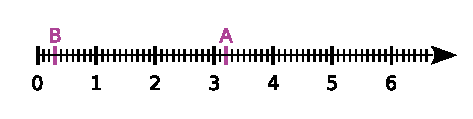
\includegraphics[width=5.5cm]{axe0BA6}
 \end{minipage}\\

Une unité est divisée en dix parts égales, ce qui signifie qu'elle est partagée en dix dixièmes. Le point $A$ se trouve 2 dixièmes à la droite du 3, donc son abscisse est $3 + 0,2 = 3,2$. De la même façon, $B$ a pour abscisse $0 + 0,3 = 0,3$. \\

  \begin{minipage}[c]{.46\textwidth}
On note $A(3,2)$ et $B(0,3)$.\\
$C(4,3) : 4,3 = 4 + 0,3$\\
$C$ se place 3 dixièmes à la droite du 4.
  \end{minipage}\hfill%
 \begin{minipage}[c]{.46\textwidth} 
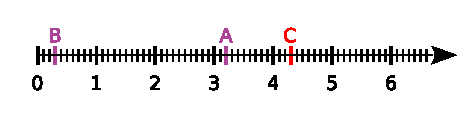
\includegraphics[width=5.5cm]{axe0BAC6}
 \end{minipage}\\

\end{exemple*1}

\exercice 

Sur une demi-droite graduée, place les points $M$ d'abscisse 2,7 et $N$ d'abscisse 5,2.
%\correction

\end{methode*1}

%%%%%%%%%%%%%%%%%%%%%%%%%%%%%%%%%%%%%%%%%%%%%%%%%%%%%%%%%%%%%%%%%%%%%%%%%%%
\begin{methode*1}[Encadrer]

\begin{aconnaitre}
\textbf{\MotDefinition{Encadrer}{}} un nombre, c'est trouver un nombre qui est plus petit que lui et un nombre qui est plus grand que lui. On écrit un encadrement avec les symboles $<$ ; $\leqslant$ ; $>$ et $\geqslant$. 
\end{aconnaitre}

\begin{exemple*1}
Encadrer 13,345 à l'unité puis au centième.\\[0.5em]
Pour encadrer à l'unité, on «coupe» le nombre 13,345 à l'unité et on obtient 13 qui est plus petit  que 13,345. Puis on ajoute \textbf{une unité}. On obtient 14 qui est plus grand que 13,345. On écrit alors : $13 < 13,345 < 14$. \\[1em]
Pour encadrer au centième, on «coupe» le nombre 13,345 au centième et on obtient 13,34 qui est plus petit que 13,345. Puis on ajoute \textbf{un centième}. On obtient 13,35 qui est plus grand que 13,345. On écrit alors : $13,34 < 13,345 < 13,35$.
\end{exemple*1}

\exercice

Encadrer les nombres 237,48 et 43,923\,5 à la dizaine puis au centième.
%\correction

\end{methode*1}

%%%%%%%%%%%%%%%%%%%%%%%%%%%%%%%%%%%%%%%%%%%%%%%%%%%%%%%%%%%%%%%%%%%%%%%%%%

\begin{methode*1}[Arrondir]

\begin{aconnaitre}
\textbf{\MotDefinition{Arrondir}{}} un nombre, c’est le remplacer par le nombre le plus proche à la précision désirée. Pour cela, on choisit le dernier chiffre à conserver puis :
\begin{itemize}
 \item on conserve ce chiffre si le suivant est 0, 1, 2, 3 ou 4 ;
 \item on augmente de 1 ce chiffre si le suivant est 5, 6, 7, 8, ou 9.
 \end{itemize}
\end{aconnaitre}

\exercice

%\correction

\end{methode*1}

%%%%%%%%%%%%%%%%%%%%%%%%%%%%%%%%%%%%%%%%%%%%%%%%%%%%%%%%%%%%%%%%%%%%%%%%%%

\section{Multiplier ou diviser}

\begin{methode*1}[Multiplier ou diviser un nombre décimal par 10 ; 100 ; 1\,000 \ldots]

\begin{aconnaitre}
\textbf{Multiplier} un nombre décimal par \textcolor{A1}{\textbf{10}}, \textcolor{B1}{\textbf{100}} ou \textcolor{J1}{\textbf{1\,000}} revient à déplacer chacun de ses chiffres vers \textbf{la gauche} de \textcolor{A1}{\textbf{1}}, \textcolor{B1}{\textbf{2}} ou \textcolor{J1}{\textbf{3}} rangs pour lui donner une valeur \textcolor{A1}{\textbf{10}}, \textcolor{B1}{\textbf{100}} ou \textcolor{J1}{\textbf{1\,000}} fois plus grande.
\textbf{Diviser} un nombre décimal par \textcolor{A1}{\textbf{10}}, \textcolor{B1}{\textbf{100}} ou \textcolor{J1}{\textbf{1\,000}} revient à déplacer chacun de ses chiffres vers \textbf{la droite} de \textcolor{A1}{\textbf{1}}, \textcolor{B1}{\textbf{2}} ou \textcolor{J1}{\textbf{3}} rangs pour lui donner une valeur  \textcolor{A1}{\textbf{10}}, \textcolor{B1}{\textbf{100}} ou \textcolor{J1}{\textbf{1\,000}} fois plus petite.
\end{aconnaitre}

\begin{remarque}
On devra parfois ajouter des zéros dans l'écriture.
\end{remarque}

\begin{exemple*1}
Effectue les calculs $6,5:100$ et $0,47 \cdot 1\,000$.\\[1em] 

\begin{minipage}{.4\linewidth}
\begin{ttableau}{.8\linewidth}{4}
\hline
 \rotatebox{90}{unités} & \rotatebox{90}{dixièmes} & \rotatebox{90}{centièmes\phantom{x}} & \rotatebox{90}{millièmes} \\ \hline
 \textcolor{B1}{\textbf{6}} , & \textcolor{B1}{\textbf{5}} & & \\ \hline
 $0\,,$ & 0 & \textcolor{B1}{\textbf{6}} & \textcolor{B1}{\textbf{5}} \\ \hline
\end{ttableau}
\end{minipage}\hfill%
%
\begin{minipage}{.55\linewidth}
Pour diviser 6,5 par \textcolor{B1}{\textbf{100}}, on déplace chacun de ses chiffres vers la droite de \textcolor{B1}{\textbf{2}} rangs et on ajoute les zéros nécessaires. 

On obtient $6,5:100 = 0,065$.

\end{minipage}
%

\vspace{2em}

%
\begin{minipage}{.4\linewidth}
\begin{ttableau}{\linewidth}{5}
\hline
\rotatebox{90}{centaines} & \rotatebox{90}{dixaines} & \rotatebox{90}{unités} & \rotatebox{90}{dixièmes} & \rotatebox{90}{centièmes\phantom{x}} \\ \hline
 & & 0 , & \textcolor{J1}{\textbf{4}} & \textcolor{J1}{\textbf{7}} \\ \hline
 \textcolor{J1}{\textbf{4}} & \textcolor{J1}{\textbf{7}} & 0 & &\\ \hline
\end{ttableau}
\end{minipage}\hfill%
%
\begin{minipage}{.55\linewidth}
Pour multiplier 0,47 par \textcolor{J1}{\textbf{1\,000}}, on déplace chacun de ses chiffres vers la gauche de \textcolor{J1}{\textbf{3}} rangs et on ajoute les zéros nécessaires. 

On obtient $0,47 \cdot 1\,000 = 470$. 
\end{minipage}
\end{exemple*1}

\exercice

Effectue : 
\begin{colenumerate}{4}
 \item $3,6 \cdot 100$ ;
 \item $870 \cdot 1\,000$ ;
 \item $63 : 10$ ;
 \item $87\,654 : 100$.
 \end{colenumerate}
%\correction
 
\exercice

Convertis en cm :
\begin{colenumerate}{4}
 \item 4 dm ;
 \item 8,1 dam ;
 \item 3,5 mm ;
 \item 0,035 m.
 \end{colenumerate}
%\correction

\end{methode*1}

%%%%%%%%%%%%%%%%%%%%%%%%%%%%%%%%%%%%%%%%%%%%%%%%%%%%%%%%%%%%%%%%%%%%%%%%%%%

\begin{methode*1}[Multiplier ou diviser un nombre décimal par 0,1 ; 0,01 ; 0,001 \ldots]

\begin{aconnaitre}
\textbf{Multiplier} un nombre décimal par \textcolor{A1}{\textbf{0,1}}, \textcolor{B1}{\textbf{0,01}} ou \textcolor{J1}{\textbf{0,001}} revient à déplacer chacun de ses chiffres vers \textbf{la droite} de 1, 2 ou \textcolor{J1}{\textbf{3}} rangs pour lui donner une valeur 10, 100 ou \textcolor{J1}{\textbf{1\,000}} fois plus petite.
\textbf{Diviser} un nombre décimal par \textcolor{A1}{\textbf{0,1}}, \textcolor{B1}{\textbf{0,01}} ou \textcolor{J1}{\textbf{0,001}} revient à déplacer chacun de ses chiffres vers \textbf{la gauche} de \textcolor{A1}{\textbf{1}}, \textcolor{B1}{\textbf{2}} ou \textcolor{J1}{\textbf{3}} rangs pour lui donner une valeur \textcolor{A1}{\textbf{10}}, \textcolor{B1}{\textbf{100}} ou \textcolor{J1}{\textbf{1\,000}} fois plus grande.
\end{aconnaitre}

\begin{remarque}
On devra parfois ajouter des zéros dans l'écriture.
\end{remarque}

\begin{exemple*1}
Effectue les calculs $2,5 \times 0,01$ et $0,65 \div 0,001$.\\[1em]

\begin{minipage}{.4\linewidth}
\begin{ttableau}{.8\linewidth}{4}
\hline
 \rotatebox{90}{unités} & \rotatebox{90}{dixièmes} & \rotatebox{90}{centièmes\phantom{x}} & \rotatebox{90}{millièmes} \\ \hline
 \textcolor{B1}{\textbf{2}} , & \textcolor{B1}{\textbf{5}} & & \\ \hline
 $0\,,$ & 0 & \textcolor{B1}{\textbf{2}} & \textcolor{B1}{\textbf{5}} \\ \hline
\end{ttableau}
\end{minipage}\hfill%
%
\begin{minipage}{.55\linewidth}
Pour multiplier 2,5 par \textcolor{B1}{\textbf{0,01}}, on déplace chacun de ses chiffres vers la droite de \textcolor{B1}{\textbf{2}} rangs et on ajoute les zéros nécessaires. 

On obtient $2,5 \times 0,01 = 0,025$.
\end{minipage}
%

\vspace{2em}

%
\begin{minipage}{.4\linewidth}
\begin{ttableau}{\linewidth}{5}
\hline
\rotatebox{90}{centaines} & \rotatebox{90}{dixaines} & \rotatebox{90}{unités} & \rotatebox{90}{dixièmes} & \rotatebox{90}{centièmes\phantom{x}} \\ \hline
 & & 0 , & \textcolor{J1}{\textbf{6}} & \textcolor{J1}{\textbf{5}} \\ \hline
 \textcolor{J1}{\textbf{6}} & \textcolor{J1}{\textbf{5}} & 0 & &\\ \hline
\end{ttableau}
\end{minipage}\hfill%
%
\begin{minipage}{.55\linewidth}
Pour diviser 0,65 par \textcolor{J1}{\textbf{0,001}}, on déplace chacun de ses chiffres vers la gauche de \textcolor{J1}{\textbf{3}} rangs et on ajoute les zéros nécessaires. 

On obtient $0,65 \div 0,001 = 650$.
\end{minipage}
\end{exemple*1}


\exercice

Effectuer :
\begin{colenumerate}{4}
 \item $5,45 \cdot 0,1$ ;
 \item $854 \cdot 0,001$ ;
 \item $63 \div 0,1$ ;
 \item $87,54 \div 0,01$.
 \end{colenumerate}
%\correction

\end{methode*1}

%%%%%%%%%%%%%%%%%%%%%%%%%%%%%%%%%%%%%%%%%%%%%%%%%%%%%%%%%%%%%%%%%%%%%%%%%%%

\begin{methode*1}[Multiplier deux nombres décimaux]

\begin{exemple*1}

Effectue la multiplication de 2,34 par 1,2.\\[1em]

On pose l'opération comme s'il s'agissait de nombres entiers. 

On effectue la multiplication de 234 par 12 sans tenir compte des virgules.

\begin{minipage}{.6\linewidth}
\begin{tabular}{rrrrcrrrr}
& 2, & 3 & 4 & $\xrightarrow{\times \text{\textcolor{B1}{\textbf{100}}}}$ & & 2 & 3 & 4 \\
$\cdot$ & & 1, & 2 & $\xrightarrow{\times \text{\textcolor{A1}{\textbf{10}}}}$ & $\cdot$ & & 1 & 2 \\ \cline{1-4} \cline{6-9}
& & & & & & 4 & 6 & 8 \\
& & & & & 2 & 3 & 4 & . \\ \cline{1-4} \cline{6-9}
2, & 8 & 0 & 8 & $\xleftarrow{\,:\,\text{\textcolor{J1}{\textbf{1\,000}}}}$ & 2 & 8 & 0 & 8 \\
\end{tabular}
\end{minipage}\hfill%
%
\begin{minipage}{.37\linewidth}
234 est \textcolor{B1}{\textbf{100}} fois plus grand que 2,34 et 12 est \textcolor{A1}{\textbf{10}} fois plus grand que 1,2. Le produit $2,34 \cdot 1,2$ est donc \textcolor{J1}{\textbf{1\,000}} fois plus petit que 2\,808. Pour obtenir le résultat, on effectue donc $2\,808 : 1\,000$.\\[0.75em]
\end{minipage}
Finalement $2,34 \cdot 1,2 = 2,808$.
\end{exemple*1}

\exercice
Sachant que $168 \cdot 32 = 5\,376$, détermine les produits (sans aucun calcul) :
\begin{colenumerate}{4}
 \item $168 \cdot 3,2$ ;
 \item $16,8 \cdot 0,32$ ;
 \item $1\,680 \cdot 3,2$ ;
 \item $1,68 \cdot 32$.
\end{colenumerate}
%\correction

\exercice

Pose et effectue les opérations :
\begin{colenumerate}{4}
 \item $68,7 \cdot 39$ ;
 \item $123 \cdot 6,3$ ;
 \item $1,3 \cdot 0,7$ ;
 \item $54,6 \cdot 8,25$.
\end{colenumerate}
%\correction

\end{methode*1}

%%%%%%%%%%%%%%%%%%%%%%%%%%%%%%%%%%%%%%%%%%%%%%%%%%%%%%%%%%%%%%%%%%%%%%%%%%%    

\begin{methode*1}[Diviser un nombre décimal par un nombre entier]

\begin{exemple*1}
Effectue la division de 75,8 par 4.\\[0.5em]

\begin{minipage}[c]{.26\textwidth}
\vspace{0em}
\begin{center}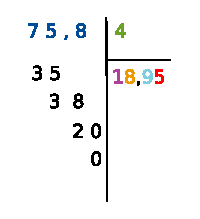
\includegraphics[width=3cm]{div758-4} \end{center}

\end{minipage}\hfill% 
\begin{minipage}[c]{.66\textwidth}

On commence par diviser la partie entière. On partage \textcolor{A1}{7} dizaines en \textcolor{H1}{4} ; le quotient comportera \textcolor{C1}{1} dizaine.\\[0.75em]
Il reste 3 dizaines. Avec les \textcolor{A1}{5} unités en plus, cela fait 35 unités à partager en \textcolor{H1}{4} ; le quotient comportera \textcolor{J1}{8} unités. \\[0.75em]
Il reste 3 unités soit 30 dixièmes. Avec les \textcolor{A1}{8} dixièmes en plus, cela fait 38 dixièmes à partager en \textcolor{H1}{4} ; le quotient comportera \textcolor{A3}{9} dixièmes. On doit donc écrire la virgule dans le quotient.\\[0.75em]
Il reste 2 dixièmes soit 20 centièmes (on a ajouté un zéro) à partager en \textcolor{H1}{4} ; le quotient comportera donc \textcolor{B2}{5} centièmes.\\[0.75em]
Ainsi $\textcolor{A1}{75,8} : \textcolor{H1}{4} = \textcolor{C1}{1}\textcolor{J1}{8},\textcolor{A3}{9}\textcolor{B2}{5}$.
\end{minipage}

\end{exemple*1}

\exercice

Calcule la valeur exacte ou une valeur arrondie au centième des quotients :
\begin{colenumerate}{4}
 \item $10 : 7$ ;
 \item $24,96 : 8$ ;
 \item $5,2 : 6$ ;
 \item $145,2 : 3$.
 \end{colenumerate}
%\correction

\end{methode*1}

%%%%%%%%%%%%%%%%%%%%%%%%%%%%%%%%%%%%%%%%%%%%%%%%%%%%%%%%%%%%%%%%%%%%%%%%%%%

\begin{methode*1}[Diviser un nombre décimal par un nombre décimal]

\begin{aconnaitre}
Le quotient de deux nombres \textbf{ne change pas} si on les multiplie (le dividende et le diviseur) par un même nombre non nul.
\end{aconnaitre}

\begin{exemple*1}
Effectue la division de 32,4 par 2,25.\\[1em]
On commence par rendre entier le diviseur en le multipliant par 100 : $2,25 \cdot 100 = 225$. On multiplie le dividende par le même nombre : $32,4 \cdot 100 = 3\,240$. On effectue la division de 3\,240  par 226, soit $3\,240 : 225 = 14,4$. On obtient ainsi le résultat de la division :

$32,4 : 2,25 = 14,4$. 
\end{exemple*1}

\exercice

Calcule la valeur exacte ou une valeur arrondie au centième des quotients :
\begin{colenumerate}{4}
 \item $4 : 6,37$ ;
 \item $13,4 : 2,45$ ;
 \item $5,87 : 2,3$ ;
 \item $0,84 : 0,12$.
 \end{colenumerate}
%\correction

\end{methode*1}

%%%%%%%%%%%%%%%%%%%%%%%%%%%%%%%%%%%%%%%%%%%%%%%%%%%%%%%%%%%%%%%%%%%%%%%%%%%        

\section{Opérations sur les durées}


%%%%%%%

\begin{methode*1}[Conversion en minutes ou en secondes]

\begin{exemple*1}

\begin{enumerate}
\item Combien y a-t-il de minutes dans 5 h 27 min ?

\begin{tabular}{ll} 
\textcolor{bleu}{\textbf{5 h}} $=$ \textcolor{bleu}{\textbf{5}} $\times$ 60 min $=$ \textcolor{bleu}{\textbf{300 min}}  & $\rightarrow$ Convertir les heures en minutes. \\
\textcolor{bleu}{\textbf{5 h}} \textcolor{vert}{\textbf{27 min}} $=$ \textcolor{bleu}{\textbf{300 min}} $+$ \textcolor{vert}{\textbf{27 min}} $=$ 327 min & $\rightarrow$ Terminer le calcul.\\
%\phantom{2 h 47 min 53 s $=$ 7\,200 s $+$ 2\,820 s $+$ 53} & \\ % phantom pour alignement avec tableau ci-dessous
\end{tabular} 

\vspace{2em}\item Combien y a-t-il de secondes dans 2 h 47 min 53 s ?

\begin{tabular}{ll} 
\textcolor{bleu}{\textbf{2 h}} $=$ \textcolor{bleu}{\textbf{2}} $\times$ 3\,600 s $=$ \textcolor{bleu}{\textbf{7\,200 s}} & $\rightarrow$ Convertir les heures en secondes. \\
\textcolor{vert}{\textbf{47 min}} $=$ \textcolor{vert}{\textbf{47}} $\times$ 60 s $=$ \textcolor{vert}{\textbf{2\,820}} s & $\rightarrow$ Convertir les minutes en secondes. \\
\textcolor{bleu}{\textbf{2 h}} \textcolor{vert}{\textbf{47 min}} 53 s $=$ \textcolor{bleu}{\textbf{7\,200 s}} $+$ \textcolor{vert}{\textbf{2\,820}} s $+$ 53 s  \\
\phantom{2 h 47 min 53 si}$=$ 10\,073 s & $\rightarrow$ Terminer le calcul. \\
\end{tabular}

\end{enumerate}
 
\end{exemple*1}

\exercice

\end{methode*1}



%%%%%%%


\begin{methode*1}[Conversion en heures, minutes et secondes]

\begin{exemple*1}
Combien y a-t-il d'heures, minutes et secondes dans 41\,000 s ? \\[1em]
\begin{minipage}[t]{.46\textwidth}
On convertit les secondes en minutes et secondes en posant la division de 41\,000 par 60 :

\begin{center}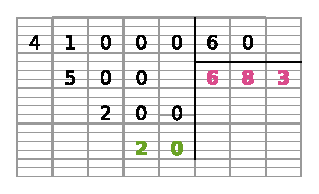
\includegraphics[width=4.6cm]{41000div60} \end{center}

On a donc 41\,000 s $=$ \textcolor{rose}{\textbf{683 min}} \textcolor{vert}{\textbf{20 s}}.
\end{minipage}\hfill%
\begin{minipage}[t]{.46\textwidth}
On convertit alors les minutes en heures et minutes en effectuant la division euclidienne de 683 par 60 :

\begin{center}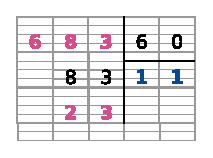
\includegraphics[width=2.9cm]{683div60} \end{center}
On a donc 41\,000 s $=$ \textcolor{bleu}{\textbf{11 h}} \textcolor{rose}{\textbf{23 min}} \textcolor{vert}{\textbf{20 s}}.
\end{minipage}


\end{exemple*1}

\exercice

\end{methode*1}

%%%%%%%%%%%%

\begin{methode*1}[Addition de durées]

\begin{exemple*1}
Un match dure 3 h 38 min et le suivant dure 2 h 49 min. Quelle est la durée totale de ces deux matchs ? \\[1em]
\begin{minipage}[t]{.34\textwidth}
On pose l'addition suivante :\\[0.2em]

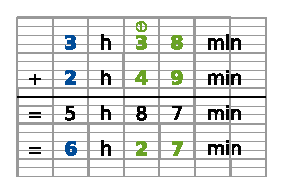
\includegraphics[width=\linewidth]{grille3h38}
\end{minipage}\hfill%
\begin{minipage}[t]{.60\textwidth}
On effectue deux additions indépendantes : 
\textcolor{vert}{\textbf{les minutes entre elles}} et \textcolor{bleu}{\textbf{les heures entre elles}}.\\[0.75em]
Mais le nombre de minutes obtenu est supérieur à 59. 
On va donc le convertir en heures et minutes sachant que 60 min $=$ 1 h. \\[0.75em]
La durée totale de ces deux matchs est donc de \textcolor{rose}{\textbf{6 h 27 min}}.
\end{minipage}

\end{exemple*1}

\exercice

Calcule :

3 h 05 min 13 s $+$ 56 min 48 s.

\vspace{1em}

1 h 46 min $+$ 2 h 37 min.

\end{methode*1}

%%%%%%%%%%%%

\begin{methode*1}[Soustraction de durées]

\begin{exemple*1}
Un film débute à 15 h 27 et finit à 18 h 14. Quelle est la durée de ce film ? \\[1em]

\begin{minipage}[t]{.34\textwidth}
On pose la soustraction suivante :\\[0.2em]

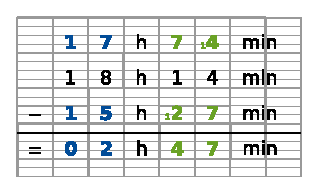
\includegraphics[width=\linewidth]{grille17h74}
\end{minipage}\hfill%
\begin{minipage}[t]{.60\textwidth}
On effectue deux soustractions indépendantes : 
\textcolor{vert}{\textbf{les minutes entre elles}} et \textcolor{bleu}{\textbf{les heures entre elles}}.\\[0.75em]
Mais on ne peut pas enlever 27 à 14. 
On va donc convertir 1 des 18 heures en 60 min. \\[0.75em]
Ce film dure donc \textcolor{rose}{\textbf{2 h 47 min}}.
\end{minipage}

\end{exemple*1}

\exercice

Calcule :

1 h 35 min 29 s $-$ 46 min 37 s.

\vspace{1em}

9 min 16 s $-$ 7 min 55 s.

%\correction

\end{methode*1}